\subsection{Security of Protocols}\label{sec:security_of_cryptographic_protocols:security}

\begin{figure}[t!]
	\begin{center}
		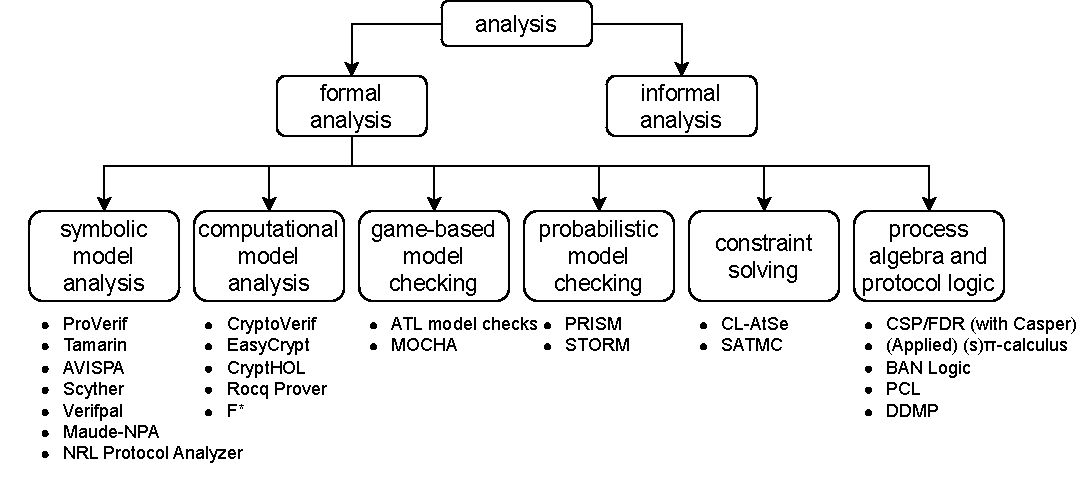
\includegraphics[width=1\linewidth]{resources/pdf/cryptographic_protocols_security_analysis_taxonomy.pdf}
		\caption{A (probably incomplete) taxonomy of methods for cryptographic protocols security analysis}
		\label{fig:cryptographic_protocols_security_analysis_taxonomy}	
	\end{center}
\end{figure}

Following the best practices described in \Cref{sec:security_of_cryptographic_protocols:design:best_practices} and watching out for the attacks listed in \Cref{sec:security_of_cryptographic_protocols:design:attacks} is not enough to claim that the design of a cryptographic protocol is secure: a security analysis is essential in that sense. The security analysis of cryptographic protocols includes (\Cref{fig:cryptographic_protocols_security_analysis_taxonomy}):
\begin{itemize}
	\item \textbf{formal methods}: mathematically rigorous and usually tool-supported, formal methods use models formalizing participants, messages, and attackers to prove security properties or find attacks by conducting exhaustive reasoning, or even pen-and-paper proofs (typically game-based proofs written in prose);
	\item \textbf{informal methods}: expert-driven and heuristic-based, informal methods rely on manual reasoning, peer review, and empirical testing.
\end{itemize}

Although being useful --- especially in early design --- informal methods lack the coverage guarantees of formal verification. Hence, formal methods are usually preferred (although complementing them with informal methods is often a good idea). For this reason, below we focus on describing the major categories of formal methods for the security analysis of cryptographic protocols (\Cref{table:security_protocols_comparison} for a high-level comparison). Note that the boundaries among the following categories may be blurred, hence a specific method may belong to multiple categories. In particular, symbolic and computational model analysis may be seen as macro-categories.

\paragraph*{Symbolic Model Analysis.} This (macro)category abstracts messages and cryptographic algorithms as symbolic terms that an attacker (usually following the Dolev-Yao threat model --- see \Cref{sec:security_of_cryptographic_protocols:design}) can manipulate but not break. In other words, symbolic model analysis is \textbf{aimed specifically at cryptographic protocols}, not cryptographic algorithms, which instead are treated as black boxes where only some properties (e.g., correctness --- see \Cref{sec:cryptography_basics:algorithms}) are preserved. For instance, symmetric encryption (\Cref{sec:symmetric_cryptography}) is often modeled with two functions \texttt{enc}($m$, $k$) and \texttt{dec}($c$, $k$) where the former stands for the encryption of a message $m$ with a key $k$, the latter stands for the decryption of a ciphertext $c$ with a key $k$, and the following equality holds \texttt{dec}(\texttt{enc}($m$, $k$), $k$) = $m$. 

\remarkBlock{Limits of symbolic model analysis}{Symbolic model analysis is suited for finding logical flaws but \textbf{cannot capture} probabilistic or complexity-theoretic aspects (e.g., brute force or cryptanalysis --- see \Cref{sec:cryptographic_security_overview:attacks}) which instead are the focus of computational model analysis.}

In symbolic model analysis, a cryptographic protocol is usually modeled through a specific language, and the resulting model is analyzed by \textbf{tools that implement automated reasoning} to search for attacks by considering all\footnote{Modern tools (e.g., ProVerif, Tamarin) use special algorithms to efficiently handle infinite state spaces --- but their execution may take a lot of time.} possible (multiple and parallel) protocol runs, messages and states,\footnote{A \textbf{state} is like a snapshot of the currently active protocol runs (including which step of their execution they reached and associated symbols), messages in transit, and the attacker's knowledge (e.g., keys, nonces, ciphertexts).} and interleavings; the final goal is to find runs (also called \textbf{traces}) that contradict security properties.

\remarkBlock{State explosion}{A common problem in symbolic model analysis is \textbf{state explosion}, that is, the rapid (and often combinatorial) growth of the number of states due to multiple/parallel/interleaved protocol runs. In other words:
	\begin{itemize}
		\item symbolic model analysis tools typically allow for an unbounded (or very large) number of protocol runs;
		\item each run creates new symbols (e.g., fresh nonces, session identifiers, and keys) that can be arbitrarily interleaved with symbols of other runs and with the attacker's actions (e.g., replaying, forging, delaying of messages);
		\item even a small number of protocol runs (<10) can produce millions of states due to interleavings and message variations.
	\end{itemize}
	As a result, symbolic model analysis may take too long or even never finish. Indeed, \textbf{the correctness of security protocols is an undecidable problem}.}

\exampleBlock{Tools for symbolic model analysis}{Major tools for symbolic model analysis are:
	\begin{itemize}
		\item \textbf{ProVerif} \cite{blanchet_efficient_2001}:\footnote{ProVerif (\url{https://bblanche.gitlabpages.inria.fr/proverif/})} widely used and state-of-the-art, supports several security properties;
		\item \textbf{Tamarin} \cite{hutchison_tamarin_2013}:\footnote{Tamarin prover: Home (\url{https://tamarin-prover.com/})} widely used and state-of-the-art, supports automated search and interactive proof steps, natively handles advanced cryptographic equational theories and global state;
		\item \textbf{Verifpal} \cite{bhargavan_verifpal_2020}:\footnote{Verifpal: Cryptographic Protocol Analysis for Students and Engineers (\url{https://verifpal.com/})} a new(er) tool aimed at students and beginners, provides an intuitive modeling language emphasizing usability to reduce user modeling errors while still performing rigorous analysis, and can export models to ProVerif for cross-verification;
		\item \textbf{AVISPA} \cite{hutchison_avispa_2005}:\footnote{AVISPA (\url{https://avispa-project.org/})} provides a common input language (HLPSL) with many back-end analyzers such as OFMC, CL-AtSe, and SATMC (historically relevant, not the state-of-the-art anymore);
		\item \textbf{Scyther} \cite{gupta_scyther_2008}:\footnote{The Scyther Tool | Cas Cremers (\url{https://people.cispa.io/cas.cremers/scyther/})} provides efficient attack discovery through pattern-based state-space search (historically relevant, not the state-of-the-art anymore).
	\end{itemize}
	Other tools not particularly relevant anymore but still worth mentioning are \textbf{Maude-NPA} and the \textbf{NRL Protocol Analyzer}.}

\paragraph*{Computational Model Analysis.} This (macro)category uses complexity theory and probabilistic reasoning to prove that any attacker with feasible resources has only a negligible probability of violating the security properties of the protocol under stated assumptions. Hence, differently from symbolic model analysis, messages are strings of bits and cryptographic algorithms (which, consequently, are functions from strings of bits to strings of bits) are not unbreakable and can only resist polynomial-time attackers under certain stated hardness assumptions (e.g., the \gls{dl} problem --- see \Cref{sec:trapdoor_functions:discrete_logarithm}).\footnote{In computational model analysis, the attacker is usually modeled as a probabilistic polynomial-time Turing machine.} As a result, computational model analysis is typically more complex, detailed, and mathematically intensive than symbolic model analysis, albeit it offers stronger security guarantees (i.e., real cryptographic security, not just logical correctness) and thus is often used by cryptographers \cite{hutchison_security_2012}.

In computational model analysis, security proofs for cryptographic protocols are usually based either on games or on simulations:
\begin{itemize}
	\item \textbf{game-based proofs} model security properties as an indistinguishability (\Cref{sec:cryptographic_security_overview:attack_model:security_goals}) or win/lose games which  --- via a series of game transformations --- are reduced to a known hard problem (e.g., the \gls{dl} problem);
	\item \textbf{simulation-based proofs} typically consist in defining an ideal functionality (that is, a specification that models perfect security) and then demonstrating that the real cryptographic protocol simulates the ideal functionality even in the presence of an attacker. A preeminent framework in this context is \gls{uc},\footnote{``Universally composable'' security --- often written as \gls{uc} security --- is the property that a given protocol satisfies within the \gls{uc} framework. In other words, \gls{uc} security is what one proves about a protocol using the \gls{uc} framework.} which provides strong composition guarantees: protocols proven \gls{uc}-secure remain secure even when composed with other protocols in arbitrary ways \cite{canetti_universally_2001}. In the \gls{uc} framework, the attacker has capabilities similar to the Canetti-Krawczyk attacker, although it is often considered to be more powerful due to its capability of performing arbitrary protocol compositions and concurrent executions. Finally, proving the \gls{uc} security of a cryptographic protocol is very complex.
\end{itemize}

\exampleBlock{Tools for computational model analysis}{Major tools for computational model analysis are:
	\begin{itemize}
		\item \textbf{CryptoVerif} (\textit{game-based}) \cite{blanchet_computationally_2008}:\footnote{CryptoVerif (\url{https://bblanche.gitlabpages.inria.fr/CryptoVerif/})} widely used, reduces security goals of cryptographic protocols to underlying mathematical problem (\Cref{sec:trapdoor_functions}), may require guidance for complex protocols;
		\item \textbf{EasyCrypt} (\textit{game-based}) \cite{aldini_easycrypt_2014}:\footnote{EasyCrypt (\url{https://www.easycrypt.info/})} supersedes CertiCrypt,\footnote{EasyCrypt/certicrypt: CertiCrypt Coq Framework (\url{https://github.com/EasyCrypt/certicrypt})} widely used, is an interactive proof assistant (i.e., less automated than CryptoVerif) tailored for cryptographic proofs, supports probability distributions, failure events, oracles, and attacker definitions, and can interact with \gls{smt} solvers (e.g., Coq) for some subgoals;
		\item \textbf{CryptHOL} (\textit{game-based}) \cite{lochbihler_crypthol_2017}:\footnote{CryptHOL - Archive of Formal Proofs (\url{https://www.isa-afp.org/entries/CryptHOL.html})} new interactive proof assistant specific for Isabelle/HOL.
	\end{itemize}
	Automation for \gls{uc} simulation-based proofs is not mature yet. Progress has been modest and often limited to specific cases, e.g., with generic proof assistants such as the Rocq Prover\footnote{Welcome to a World of Rocq (\url{https://rocq-prover.org/})} --- formerly known as Coq --- Isabelle/HOL,\footnote{Isabelle (\url{https://isabelle.in.tum.de/})} and F*,\footnote{F*: A Proof-Oriented Programming Language (\url{https://fstar-lang.org/})} which are highly rigorous but require significant manual effort and expertise.
}

\paragraph*{Game-Based Model Checking.} This category models protocol analysis as a two-player game on a state graph. In this case, ``game-based'' refers to modeling a cryptographic protocol and the attacker within a state-transition system, then using temporal logic model checking to verify strategy-dependent security properties (e.g., fairness, timing) expressed as game objectives. 

\exampleBlock{Tools for game-based model checking}{An influential formalism for game-based model checking tools is \gls{atl} \cite{alur_alternating_2002}, while a notable tool is \textbf{MOCHA} \cite{goos_mocha_1998}.\footnote{MTC (Models and Theory of Computation): Mocha Project (\url{https://ptolemy.berkeley.edu/projects/embedded/research/mocha/})}}

\paragraph*{Probabilistic Model Checking.} This category is an extension of traditional model checking for probabilistic state machines or Markov decision processes, and consists in quantifying probabilities in finite or parameterized models for anonymity, randomness, or performance-security trade-offs. 

\remarkBlock{Probabilistic model checking for cryptographic protocols}{Probabilistic model checking of cryptographic protocols usually requires abstracting cryptography to small probability events (since real cryptographic probabilities are negligible but not exactly zero). For this reason, probabilistic model checking is more common in the analysis of privacy protocols (onion routing, mixing networks) and quantum cryptography protocols, where randomness and probability are intrinsic and the properties (like ``anonymity level'' or ``key distribution success rate'') are quantitative.}

\exampleBlock{Tools for probabilistic model checking}{Notable tools for probabilistic model checking are \textbf{PRISM} \cite{gopalakrishnan_prism_2011}\footnote{PRISM - Probabilistic Symbolic Model Checker (\url{https://www.prismmodelchecker.org/})} and \textbf{Storm} \cite{hensel_probabilistic_2022}.\footnote{Storm -- A Modern Probabilistic Model Checker -- Home (\url{https://www.stormchecker.org/})}}

\paragraph*{Constraint Solving.} This category consists in reducing security analysis to logical constraints analysis: rather than exploring all traces, constraint solving encodes the existence of an attack trace as a satisfiability problem. Constraint solving is often an integral part of automated analyzers (e.g., AVISPA, Tamarin).

\exampleBlock{Tools for constraint solving}{Notable tools for constraint solving are \textbf{CL-AtSe} \cite{hutchison_clatse_2006} and \textbf{SATMC} \cite{hutchison_satmc_2014}.\footnote{SATMC - Security \& Trust (\url{https://st.fbk.eu/tools/SATMC/})}}

\paragraph*{Process Algebra and Protocol Logic.} This category relies on formal languages to model and analyze protocols: although representing a concept on its own, \textbf{process algebra}\footnote{In general, an algebra is a mathematical structure including a set of values, a set of operations on these values, and possibly algebraic properties such as commutativity and associativity. In a process algebra, processes are values and parallel composition is a commutative and associative operation on processes --- see \url{https://www.cs.tufts.edu/~nr/cs257/archive/jeannette-wing/pi.pdf}.} and protocol logic are often used as a modeling foundation for automated analyzers. Process algebra describes concurrent interactions and message flows, while protocol logic uses logical systems tailored to security.

\exampleBlock{Formalisms for process algebra and protocol logic}{An influential formalism for process algebra is $\pi$-calculus (and its extensions applied $\pi$-calculus and spi-calculus\footnote{The Spi Calculus (\url{https://piazza.com/class_profile/get_resource/hzdnubyxvfx3sg/i3rz8bcdpsdwi})} tailored for cryptographic protocols \cite{abadi_calculus_1997}), while an influential formalism for protocol logic is the \gls{ban} logic (more popular in the past) \cite{burrows_logic_1990} and the \gls{pcl} \cite{datta_protocol_2007}.}

\readBlock{More information on $\pi$-calculus}{Jeannette M. Wing's document ``FAQ on $\pi$-Calculus'' --- available at the link \url{https://www.cs.tufts.edu/~nr/cs257/archive/jeannette-wing/pi.pdf} --- is a good primer on $\pi$-calculus.}

The aforementioned categories often complement, generalize, and build upon each other (e.g., tools for symbolic methods are often based on constraint solving). More importantly, their application is not limited to the security analysis of cryptographic protocols; in that regard, \textbf{symbolic methods} are the easiest and excel at rapid automated analysis under idealized assumptions, while \textbf{computational methods and process algebra} provide higher assurance with greater effort. Specialized formal methods (e.g., game-based model checking, probabilistic verification, and protocol logic) address niches that general tools might not cover (e.g., fairness, anonymity). 

\warningBlock{Important limitations of formal methods}{Formal methods often produce models of cryptographic protocols and, by definition, models abstract many real-world issues. Hence, important concerns in applied cryptography (e.g., key management, side-channels attacks, programming languages, \gls{tcb} --- see \Cref{sec:key_management,sec:security_of_cryptographic_algorithms,sec:programming_languages_and_software}), which lie outside the scope of formal methods, should still be considered and addressed properly.}

\readBlock{More information on techniques for verification of cryptographic protocols}{The article ``Security Protocol Verification: Symbolic and Computational Models'' \cite{hutchison_security_2012} provides a survey of techniques for analyzing the security of cryptographic protocols with symbolic and computational model analysis as well as verifying the security of protocols implementations.}

\begin{table}[!b]
	\centering
	\scriptsize
	\setlength{\tabcolsep}{3pt}
	\def\arraystretch{1.075}
	\rowcolors{0}{white}{cloud}
	\caption{High-level comparison of formal methods categories for investigating the security of cryptographic protocols. Please note that the table is a simplification and the information it contains may be approximate and surely not comprehensive}
	\newcolumntype{Y}{>{\centering\arraybackslash}X}
	\begin{tabularx}{\textwidth}{l|ccYYY}
		
		\toprule
		
		\multicolumn{1}{c|}{\textbf{category}} & 
		\multicolumn{1}{c}{\textbf{Automation}} &
		\multicolumn{1}{c}{\textbf{Scalability}} &
		\multicolumn{1}{c}{\textbf{Expressiveness}} &
		\multicolumn{1}{c}{\textbf{Most suitable for}} &
		\multicolumn{1}{c}{\textbf{Adoption}} \\
		
		\hline
		
		\textbf{symbolic} 					& high & high & logic (symbolic) & design-stage & widespread \\
		\textbf{computational (game)} 		& medium/low & medium/low & hardness assumptions & high assurance & academic \\
		\textbf{computational (\gls{uc})}	& low & low & extremely expressive & protocol composition & niche \\
		\textbf{game model checking} 		& high & medium & strategic properties & fairness & niche \\
		\textbf{prob. model checking}		& high & medium & probabilistic events & quantitative security & niche in academic \\
		\textbf{constraint solving}			& high & high & algebraic properties & attack discovery & ~widespread \\
		\textbf{process algebra and} 		& medium & medium & extremely expressive & refinement and & academic \\
		\rowcolor{cloud}
		\textbf{protocol logic}				& (may vary) & & (may vary) & sub-protocol analysis & \\
		
		\bottomrule
		
	\end{tabularx}
	\label{table:security_protocols_comparison}
\end{table}
